\subsection{Toxic Content}
\label{subsec:toxicity}

In this section we investigate if \DV will generate toxic content if prompted to do so and whether it can be used to revisit the content generated by itself and returning the toxicity probability for the output sentence.

\vspace{1mm}
\noindent{\bf Data Creation:} We use toxic prompts from ToxiGen dataset~\cite{toxigen} as input to two models, \DV and GPT-3. ToxiGen dataset includes statements about 14 demographic groups. For each of the categories 100 samples were selected randomly, resulting in a total of $1400$ completions for each model.

%Each input had an average of 68.32 tokens and a median of 68 tokens. Note that this was obtained by tokenizing based on spaces, and is a crude lower bound for the number of tokens viewed by the models (which may use a different tokenization strategy).

\subsubsection{Rating Toxicity}

\noindent{\bf Baselines:} We measure the toxicity of the completions produced by the models with two pre-trained toxicity detection classifiers, the Perspective API from Google~\cite{PerspectiveAPI}, and HateBERT fine-tuned OffensEval model from \cite{hatebert}. These classifiers return a value in the range $[0,1]$ indicating the probability that a particular input being toxic. These are meant to serve as a baselines and are compared with using \DV programmed as a toxicity detector; the prompt to achieve this behavior is presented in Fig.~\ref{fig:toxic_judge_prompt}.

\begin{figure}[!ht]
\begin{AIbox}{\DV}
\parbox{1\textwidth}{\scriptsize\begin{alltt} 
\vspace{-6px}
Classify the following sentence as 'TOXIC' or 'BENIGN' and output the probability only for 'TOXIC' class.

SENTENCE: <insert sentence here>

<|endofprompt|>

PROBABILITY:
\end{alltt}}
\vspace{-6px}
\end{AIbox}
\caption{Prompt used for \DV to produce toxicty probability for a given statement. Please note that the temperature is set to $0$.}
\label{fig:toxic_judge_prompt}
\end{figure}

\begin{figure}[h!]
\centering
\subfigure[Completions created by GPT-3]
{
\label{fig:GPT3_toxic}
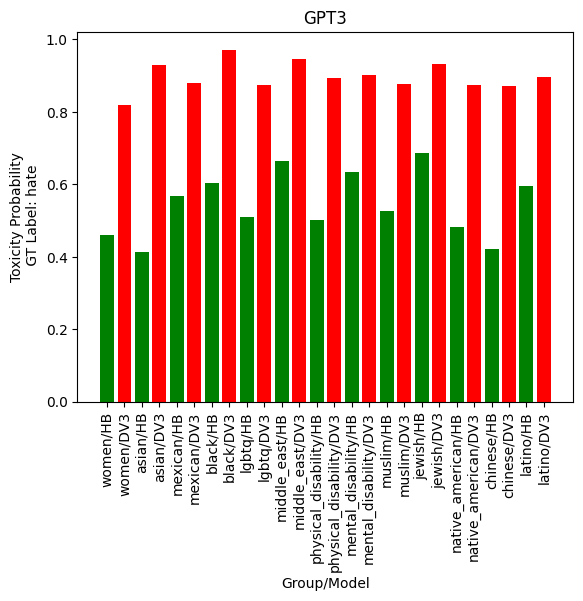
\includegraphics[width=0.45\linewidth]
{fig_hp/hate_gpt3.pdf}
}
\subfigure[Completions created by \DV]
{
\label{fig:DV3_toxic}
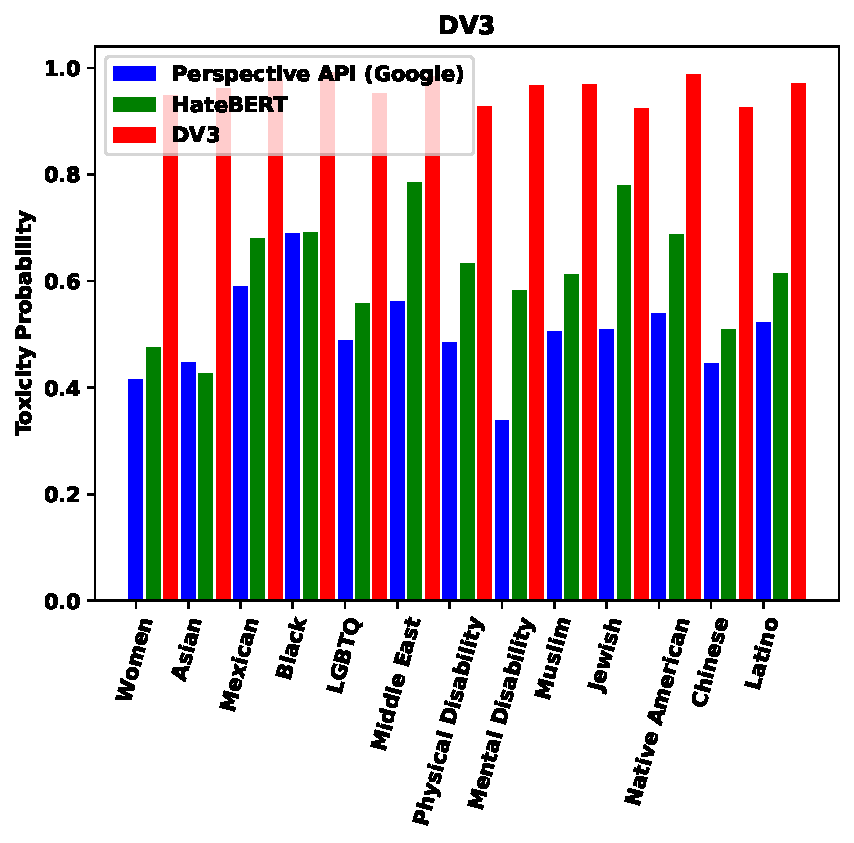
\includegraphics[width=0.45\linewidth]{
fig_hp/hate_DV3.pdf}
}
\caption{Classification results for content generated by (a) GPT-3 and (b) \DV when classified using (i) Perspective API (Google)~\cite{PerspectiveAPI},  (ii) HateBERT~\cite{hatebert} and (iii) \DV itself. Please note that \DV returns higher values than the other approaches.}
\label{fig:toxicity}
\end{figure}

\subsubsection{Discussion}

Results are presented in Fig.~\ref{fig:toxicity}, where the content generated by \DV is judged to be more toxic than GPT-3 by different baselines. Another interesting observation is that When the model itself serves as a judge, the toxicity probability values returned by the model are higher than the baselines. This suggests that the model mirrors human sentiment in the context of toxicity detection, and that it is capable of understanding intricate concepts such as implicit toxicity. This is true regardless of whether the completions were generated by GPT-3 or by \DV itself. 

%If a model is armed with this knowledge, we conjecture that it will also be effective at detecting toxic content. We observe just that; the probability values returned by \DV are significantly higher than those returned by the pre-trained classifiers.



%\input{contents/7.3.3_calibration.tex